% The first command in your LaTeX source must be the \documentclass command.
\documentclass[sigconf]{acmart}
\usepackage{listings}
\usepackage{dirtytalk}
\usepackage[shortlabels]{enumitem}
\usepackage{amssymb}
\usepackage{minitoc}
\usepackage{algorithm}
\usepackage[noend]{algpseudocode}
\usepackage{mathtools}

% pseudocode
\algnewcommand\algorithmicforeach{\textbf{for each}}
\algdef{S}[FOR]{ForEach}[1]{\algorithmicforeach\ #1\ \algorithmicdo}

\DeclarePairedDelimiter{\ceil}{\lceil}{\rceil}


%
% \BibTeX command to typeset BibTeX logo in the docs
\AtBeginDocument{%
  \providecommand\BibTeX{{%
    \normalfont B\kern-0.5em{\scshape i\kern-0.25em b}\kern-0.8em\TeX}}}

% Rights management information. 
% This information is sent to you when you complete the rights form.
% These commands have SAMPLE values in them; it is your responsibility as an author to replace
% the commands and values with those provided to you when you complete the rights form.
%
% These commands are for a PROCEEDINGS abstract or paper.
\copyrightyear{2020}
\acmYear{2020}
\setcopyright{acmlicensed}
\acmConference[KDD-ADS '20]{KDD-ADS '20: Knowledge Discovery and Data Mining - Applied Data Science 2020}{August 22th, 2020}{San Diego, California, USA}
\acmBooktitle{KDD-ADS '20: Knowledge Discovery and Data Mining - Applied Data Science 2020, August 22th, 2020, San Diego, California, USA}
\acmPrice{15.00}
\acmDOI{10.1145/1122445.1122456}
\acmISBN{978-1-4503-9999-9/18/06}

%
% These commands are for a JOURNAL article.
%\setcopyright{acmcopyright}
%\acmJournal{TOG}
%\acmYear{2018}\acmVolume{37}\acmNumber{4}\acmArticle{111}\acmMonth{8}
%\acmDOI{10.1145/1122445.1122456}

%
% Submission ID. 
% Use this when submitting an article to a sponsored event. You'll receive a unique submission ID from the organizers
% of the event, and this ID should be used as the parameter to this command.
%\acmSubmissionID{123-A56-BU3}

%
% The majority of ACM publications use numbered citations and references. If you are preparing content for an event
% sponsored by ACM SIGGRAPH, you must use the "author year" style of citations and references. Uncommenting
% the next command will enable that style.
%\citestyle{acmauthoryear}

%
% end of the preamble, start of the body of the document source.
\begin{document}

%
% The "title" command has an optional parameter, allowing the author to define a "short title" to be used in page headers.
\title{Lightweight Real-Time Feature Monitoring}

%
% The "author" command and its associated commands are used to define the authors and their affiliations.
% Of note is the shared affiliation of the first two authors, and the "authornote" and "authornotemark" commands
% used to denote shared contribution to the research.
\author[Conde]{João Conde}
\email{joao.conde@feedzai.com}
\affiliation{%
  \institution{Feedzai}
}

\author[Sampaio]{Marco O. P. Sampaio}
\email{marco.sampaio@feedzai.com}
\affiliation{%
  \institution{Feedzai}
}

\author[Cardoso]{Pedro Cardoso}
\email{pedro.cardoso@feedzai.com}
\affiliation{%
	\institution{Feedzai}
}

\author[Restivo]{André Restivo}
\email{arestivo@fe.up.pt}
\affiliation{%
	\institution{University of Porto}
}

\author[Ribeiro]{Pedro Ribeiro}
\email{pribeiro@dcc.fc.up.pt}
\affiliation{%
  \institution{University of Porto}
}


    


%
% By default, the full list of authors will be used in the page headers. Often, this list is too long, and will overlap
% other information printed in the page headers. This command allows the author to define a more concise list
% of authors' names for this purpose.
%\renewcommand{\shortauthors}{Trovato and Tobin, et al.}

%
% The abstract is a short summary of the work to be presented in the article.
\begin{abstract}
Many real-time stream monitoring systems are static once deployed in a production environment. Over time, due to data pattern shifts, the initially deployed static system's performance gradually deteriorates. Accurate and timely detection of data pattern deviations allow for immediate measures to be taken. Thus, the problem at hand is to determine when to reconfigure the system, \textit{e.g.}, a Machine Learning model, based on an analysis of the drifts in the stream of data. In this paper, we present a method that makes use of constant time and memory streaming aggregations and distribution divergence functions to alert deviations in data patterns in real-time. We generate alerts based on a user-defined probability threshold, for each of an event's numerical fields, denominated features in our context. We evaluate our method through a series of tests, some with synthetic data sets and some with real data. We further split the tests into single and multi-feature analysis. Our method accurately detected the introduced anomalies in the experiments using synthetic datasets while maintaining high throughput, for single and multi-feature analysis. However, experiments with real data were not as accurate. Despite not knowing the specific reasons for that, we detail further investigation to future work and formulate a set of hypotheses that might explain the latter results and hence are worthy of pursuing next.
\end{abstract}

%
% The code below is generated by the tool at http://dl.acm.org/ccs.cfm.
% Please copy and paste the code instead of the example below.
%
\begin{CCSXML}
<ccs2012>
   <concept>
       <concept_id>10002951.10003227.10003351.10003446</concept_id>
       <concept_desc>Information systems~Data stream mining</concept_desc>
       <concept_significance>500</concept_significance>
       </concept>
   <concept>
       <concept_id>10010520.10010570.10010574</concept_id>
       <concept_desc>Computer systems organization~Real-time system architecture</concept_desc>
       <concept_significance>500</concept_significance>
       </concept>
 </ccs2012>
\end{CCSXML}

\ccsdesc[500]{Information systems~Data stream mining}
\ccsdesc[500]{Computer systems organization~Real-time system architecture}

%
% Keywords. The author(s) should pick words that accurately describe the work being
% presented. Separate the keywords with commas.
\keywords{data streams, monitoring, real-time, lightweight, concept drift}


%
% This command processes the author and affiliation and title information and builds
% the first part of the formatted document.
\maketitle

\section{Introduction}
In the past decade, applications have become increasingly data-driven, placing data at the center of application design. For different use cases, the data is processed in different ways for different purposes. For instance, e-commerce platforms such as Alibaba need to process a large number of daily transactions while ensuring that sales run smoothly and that products are delivered to customers' homes. Streaming services, like YouTube and Netflix, try to guarantee that media content reaches up to millions of users simultaneously. Social networks are responsible for generating large volumes of data. Twitter, for example, generates more than 500 million \textit{tweets} (posts in Twitter) per day. \textit{Tweets} may contain text, media content or both. Cybersecurity applications are yet another example of time-sensitive, data-driven applications. The entities that work in these use cases need to monitor user accesses and their actions in the network, where timely detection of intruders is critical to prevent them from tampering with the underlying system.

All of these applications generate large volumes of data which lead to the creation of multiple real-time unbounded datasets, also known as data streams. The information that flows through such a stream can be analyzed on-the-fly or stored for later processing. The former is best known as stream processing, whereas the latter is known as batch processing. Streaming data is known for being non-stationary \cite{Gama-Knowledge-Discovery} where the value of the produced information lies in its recency \cite{Kolajo-Big-data-stream-SLR}. \textit{Recency} is measured under different scales for different use cases. For instance, consider the monitoring of geological data to forecast possible natural disasters such as earthquakes versus the monitoring of a computer network for intruder detection. In the former case, after the forecast of a future earthquake, governmental authorities need a couple of days to launch an evacuation plan and keep the population safe. However, in the intruder detection scenario, the decision of removing access to a user must be done as soon as possible, preferably in a few seconds. Hence, while in the first scenario information retrieved within a day would still be recent, in the second scenario, information is considered recent and relevant if delivered within seconds (or even milliseconds).

Consider the use case where we want to detect credit card fraud on the data stream of all the transactions made on Amazon by every US citizen on a single day. In this case, Amazon's transaction stream will need to be monitored by another system, a fraud detection one. Such a system would have to process all incoming transactions and decide, in a fraction of a second, if a transaction is fraudulent or not. Unlike the fraud detection system, our system is not mission-critical. Hence, it must monitor the data stream looking for data pattern deviations in real-time but with a low memory footprint.

In this paper, we present a lightweight real-time system that monitors a stream of high volumes of high velocity, highly skewed and seasonal data and detects pattern shifts relative to a reference period. The motivation to detect data stream pattern deviations in real-time is to know when to reconfigure the mission-critical system (\textit{e.g.}, retrain the Machine Learning model) before its performance decays. We want to build a lightweight enough solution that can be integrated into existing workflows since having a real-time system monitoring other real-time systems consuming as many resources as the latter would be far too costly.

\section{Related Work}
\label{sec:RelatedWork}


\section{Method}
\label{sec:Method}
A data stream is a continuous collection of events, each timestamped and with multiple fields. In this paper, we refer to the event's fields as features. Our goal is to detect data pattern deviations for each feature in a streaming fashion. To that end, we devise a method that works with two windows and comprises two phases, a batch analysis phase and a stream analysis one. The batch analysis is performed on a static in time window which we call the reference window. The stream analysis is performed over an emulated sliding window that groups data stream events. We aggregate the contents of the reference window with an exact histogram and the sliding window with an approximate histogram aggregation based on Exponential Moving Averages (EMAs). We then apply a statistical distribution divergence function to both histogram aggregations to obtain a divergence value. In the batch phase, we build the distribution of these values so we can define a percentile threshold for the newly measured divergence values in streaming. We raise alerts for features above certain percentiles, \textit{e.g.}, the 99th percentile.

\subsection{EMA-based histogram} \label{sec:ema-hist}
Exponential Moving Averages (EMAs) \cite{EMA-Everett2011, EMA-Hunter, EMA-MarcusB} are a type of reduce functions applied to a sequence of elements in an orderly fashion to compute a weighted average, using different weights for each element. These weights decrease exponentially with the age of the observations. EMAs are recursive: $EMA_t$ depends only on the $val_t$ plus a smoothed $EMA_{t-1}$. This recursive property allows us to store only one EMA value and continuously update it for each new value $val_t$, based on the following recursion formula:
\begin{definition}
EMA\textsubscript{t} = EMA\textsubscript{t-1} * $2^{-\frac{1}{n_{1/2}}}$ + $val_t$
\label{def:tuple-ema}
\end{definition} where $n_{1/2}$ is the tuple-based half-life of the EMA. 
The half-life $n_{1/2}$ controls how fast old events are forgotten. The tuple-based half-life is the amount of tuples or events the EMA must process before a certain element has its weight reduced by half. For example, with a tuple-based half-life of $n_{1/2}=1$ tuple, for each new tuple, all weights are reduced by half. 

Each count of our EMA-based histogram is essentially an EMA-count. Algorithm \ref{pseudo:ema-hist} shows how we update our EMA histogram. We assume we have access to global \textit{counts} and \textit{bins} arrays and use a suppression factor of $2^{- \frac{1}{n_{1/2}}}$. The histogram aggregation is updated for each new streaming value \texttt{val} using the \texttt{processValue(val)} function, that increments the correct histogram bin (note that the \textit{bins} array defines the bin boundaries while the \textit{counts} array actually holds each bin's count) and applies the EMA suppression to every bin.
\begin{algorithm}[!htb]
    \caption[EMA histogram]{EMA histogram sliding window emulation}
    \label{pseudo:ema-hist}
    \begin{algorithmic}[1]
        \Function{getBin}{val}
            \State \Return{binarySearch(bins, val)}
        \EndFunction
        
        \Function{processValue}{val}
            \State $bin \gets getBin(val)$
            \State $counts[bin] \gets counts[bin] + 1$ \Comment{//Increment correct bin}
            
            \ForEach {$count \in counts$} \Comment{//EMA suppression}
                \State $count \gets count \times 2^{- \frac{1}{n_{1/2}}}$
            \EndFor
        \EndFunction
    \end{algorithmic}
\end{algorithm}
This procedure is illustrated in Figure \ref{fig:EMA-hist-build}.
\begin{figure}[!htb]
    \begin{center}
    %\hspace{6cm}
      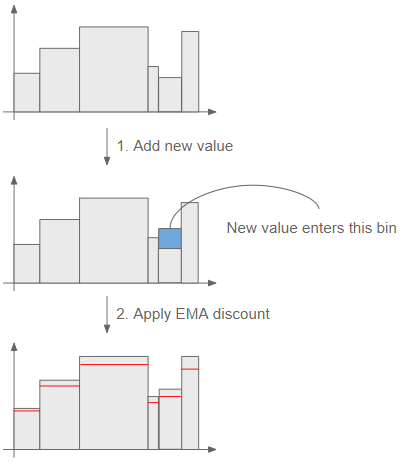
\includegraphics[scale=0.6]{figures/ema-hist.png}
      \caption[]{Reference equal-height histogram}
      \label{fig:EMA-hist-build}
    \end{center}
\end{figure}

The EMA-based approximate histogram emulates a sliding window as an exponential tail. This aggregation shows constant memory and time complexity regarding window size, making it ideal for our lightweight real-time system.

\subsection{Batch Analysis Phase} \label{sec:batch-phase}
The main goals of the batch phase are to build our reference aggregation and the distribution of divergence values, for each feature. Streaming divergence values will be compared to this distribution of values later to find out how probable a value is to occur (if it is very low, an alert is raised).

\subsubsection{Building the Reference Histogram}
First, for each feature, we compute the reference histogram from the reference period. When building it we ensure the histogram has equal counts for all bins which results in different sized bins. Equal height histograms adjust better to wildly varying distributions. Equal height means we have more bins covering very dense regions and fewer bins in lower density regions. 

\subsubsection{Building the Distribution of Divergence Values} \label{sec:sampling-batch}
Secondly, we aim to build the distribution of expected distance or divergence values, to later on threshold the observed distance values during the streaming phase. To that end, we make $S$ samples of transactions, each with the same tuple-based size of the sliding window we emulate in streaming. Each sample is a contiguous block of transactions, thus preserving the order of transactions and the time-dependency property of a time-series. With this sampling we aim to build a distribution of divergence values and reliably estimate the upper tail of that distribution. In \cite{SAMM}, the authors show how many samples must be made to have at least one value in the upper tail of the distribution. Defining $\alpha$ as our threshold and $\frac{\alpha}{n_{features}}$ as our threshold corrected by the Holm Bonferroni multiple test correction, $\gamma$ is defined as the probability of \textbf{not} having at least one point in the $\frac{\alpha}{n_{features}}$ upper tail of the distribution and the minimum number of samples $S$ to make is given by:
\begin{equation*}
    \label{eq:optimal-n-samples}
    \textit{S} = \ceil[\bigg]{\frac{\log\gamma}{log(1 - \frac{\alpha}{n_{features}})}}
\end{equation*}
For each sample, and each feature, we compute the approximated EMA histogram using the bins from the reference histogram. We also add two extra bins that will cover the region to the left and the right of our histogram, respectively. This way, observed values outside of the reference period will be placed in these special bins, either left or right. We compute multiple sample histograms to encode distributions over smaller time periods that may exist within the large reference period. We use an approximated histogram to mimic the target approximated histogram we will incrementally maintain in the streaming environment.

For each feature, we have now \textit{S} histograms, one for each sample. We compute the divergence between each of the \textit{S} histograms and the reference histogram. Figure \ref{fig:compute-sample-distances} illustrates this process as we apply our divergence or distance function for each sample's EMA-based histogram and the reference histogram, obtaining \textit{S} divergence measurements.
\begin{figure}[!htb]
    \begin{center}
      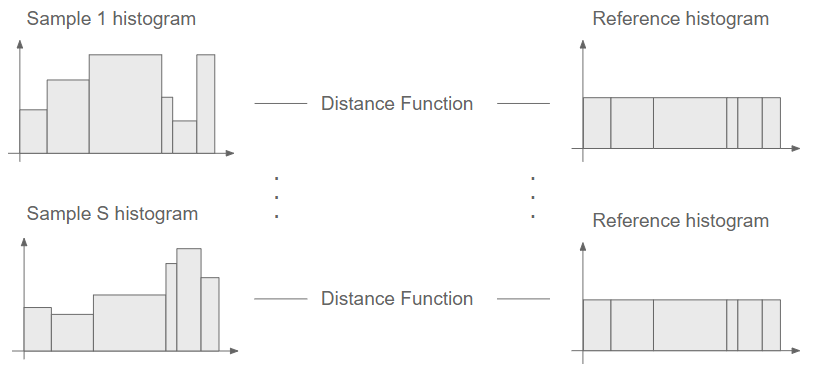
\includegraphics[scale=0.4]{figures/compute-sample-distances.png}
      \caption[Compute sample's distance values]{Compute divergence values between reference and samples}
      \label{fig:compute-sample-distances}
    \end{center}
\end{figure}
These $S$ measurements are divergence measurements between random samples of data and the reference period. Hence, we claim we now know the distribution of expected distance values. Given a new distance value measured between another random window and the reference window, we can compute its probability and produce alerts if the probability is below a certain threshold. Note that the histograms for each sample are EMA-based histograms just like the emulated sliding window histogram. This ensures a certain degree of fidelity in the test we make in streaming because we measure the divergence between a random sample of data (our streaming histogram or any of the sample's histogram) and the reference one.

\subsubsection{Burn-In Period at System Initialization}
When we boot up our system in the streaming phase we initially have empty histogram aggregations. To avoid this burn-in period, we propose saving the last sample's histogram for each feature so that the sliding window EMA-based histogram aggregation is initialized with it.

\subsubsection{Batch Phase Artifacts} \label{sec:batch-artifacts-summary}
By the end of the batch phase, for each feature, we have: 
\begin{enumerate}
    \item a reference histogram
    \item a distribution of divergence values
    \item the last sample's histogram
\end{enumerate}


\subsection{Streaming Phase} \label{sec:stream-phase}
In the streaming phase, the system will process event by event and perform a change detection test periodically. For each feature, we initialize the approximate histogram with the last sample's data, from the batch phase. Then, for each incoming event and each of the event's features, we update our streaming approximate histogram for that feature by adding the new value and then "cutting a slice" from the top of the histogram bars to simulate eviction, as described in Section \ref{sec:ema-hist}. This is all we do, regarding event processing.

We periodically perform a multi-feature change detection test. The test is done by first computing the divergence between the reference histogram for a feature \textit{x} and the sliding window EMA-based histogram of the same feature. This value is tested against the known distribution of distance values for feature \textit{x}. We test to see if the percentile of the computed distance relative to the distribution of divergence is above a certain percentile. The probability of a divergence value $val_x$ (or \textit{p-value}) is:
\[pvalue(val_x) = 1 - percentile(val_x)\]
For example, if we define alerts to have 1\% or less probability to happen, it means the system will raise an alert for distance values above the 99th-percentile or \textit{p-value} = 0.01. We alert a feature \textit{x} as divergent at a given timestamp if for a given probability threshold $\alpha$:
\[ percentile(val_x) > 1 - \alpha \]
or:
\begin{equation}
    \label{eq:alert-test}
    pvalue(val_x) < \alpha
\end{equation}

\subsubsection{Multiple Test Correction} \label{sec:multi-test}
Note that we periodically apply this test (Equation \ref{eq:alert-test}) for each feature, effectively repeating the analysis. When considering several hypotheses, the problem of multiplicity arises \cite{MultiTestProblem-Pubmed, MultiTestProblem-Dickhaus2014, MultiTestProblem-Miller1966, multiple-test-correction-geoffrey}: the more hypotheses are checked, the higher the probability of obtaining false positives. In the literature, many multiple test correction methods are proposed, but we opted to use the Holm-Bonferroni multiple test correction because it is a simple and easy to compute correction that can reduce the number of false negatives while having as target to control the number of false positives. Furthermore, it does not require to assume any independence between the tested hypothesis (as other methods do) which would almost surely be a wrong assumption for realistic datasets. In statistics, the Family-Wise Error Rate (FWER) \cite{MultivariateMT, MultitestTamhane2018AdvancesIP} is the probability of having one or more false positives when performing multiple hypotheses tests, \textit{i.e.}, considering one hypothesis true when it is not. The Holm-Bonferroni method \cite{HolmBonferroni} is one of many approaches for controlling the Family-Wise Error Rate \textit{(FWER)} by adjusting the rejection criteria for each hypothesis.


\subsubsection*{Holm-Bonferroni Correction} \label{sec:holmbonferroni}
The Holm-Bonferroni correction takes Equation \ref{eq:alert-test} and corrects the right-side threshold $\alpha$ for each feature. This correction is done by dividing the threshold $\alpha$ by a correction factor. First, we compute the \textit{p-value} of each feature. We then order our features by \textit{p-value}, in ascending order. Next, starting from the first feature, the one with the smallest \textit{p-value}, and proceeding until the end of the list of features, we check if:
\begin{equation}
    pvalue(val_x) < \alpha / (m - k)
    \label{eq:corrected-pvalue}
\end{equation}
with $\alpha$ as the probability to reject the null hypothesis, \textit{m} as the number of hypotheses to test (in our case the number of features) and \textit{k} as the 0-based index of the current feature. We stop at the first feature that fails this test, and every feature processed up until this one is considered to be a divergent feature and alerts are raised.


\section{Experiments}
\label{sec:Experiments}

Much scientist

\section{Discussion}
\label{sec:Discussion}

Fight

\section{Conclusions}
\label{sec:Conclusions}
Thesis done, PogU

\bibliographystyle{ACM-Reference-Format}
\bibliography{myrefs.bib}

\end{document}
